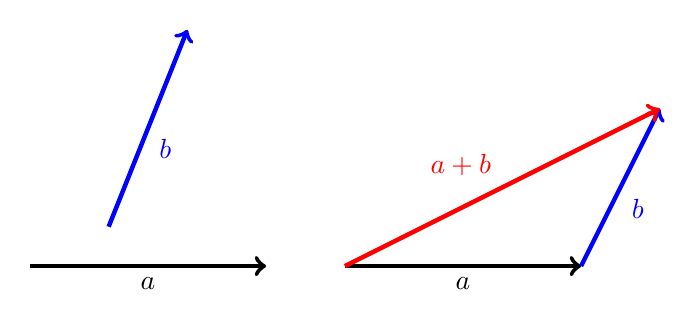
\begin{tikzpicture}
\draw [->, ultra thick] (-1, -1) -- (2, -1) node[midway,below] {$\boldsymbol{a}$};
\draw [shift={(4, 0)}, ->, ultra thick, ] (-1, -1) -- (2, -1) node[midway,below] {$\boldsymbol{a}$};
\draw [->, ultra thick, color = blue] (0, -0.5) -- (1, 2) node[midway,below right] {$\boldsymbol{b}$};
\draw [shift={(6, -1)}, ->, ultra thick, color = blue] (0, 0) -- (1, 2) node[midway,below right] {$\boldsymbol{b}$};
\draw [->, ultra thick, color = red] (3, -1) -- (7, 1) node[midway,above left] {$\boldsymbol{a}+\boldsymbol{b}$};
\end{tikzpicture}
